\section{System design}

\subsection{Summary of the design}


\begin{center}
Table 21. Objectives and boundary conditions\\
\begin{tabular}{ |l|c| } 
\hline
\textbf{Parameter} & \textbf{Value/Description}  \\ 
\hline
Onshore or Offshore & Onshore  \\ 
\hline
Type of location & Shrubs \\ 
\hline
Wind conditions: Weibull scale factor & 7.5734 \\
\hline
Wind conditions: Weibull shape factor & 2.1416 \\
\hline
Noise constraint (max tip speed) & 72.497 m/s \\
\hline
Visual constraint & - \\
\hline
\end{tabular} \\
\end{center}

\begin{center}
Table 22. Design variables/choices\\
\begin{tabular}{ |l|c| } 
\hline
\textbf{Parameter} & \textbf{Value/Description}  \\ 
\hline
Rated power & 2 MW  \\ 
\hline
Number of blades & 3 \\ 
\hline
Rotor diameter & 96.4 m \\
\hline
Design tip speed ratio & XX \\
\hline
Rotational speed range & XX \\
\hline
Cut-in wind speed & XX \\
\hline
Cut-out wind speed & XX \\
\hline
Rated wind speed & XX \\
\hline
Hub height & XX \\
\hline
\end{tabular}
\end{center}

\subsection{Supporting material, analyses and rationale}

The wind turbine designed and described in this report is made for \textcolor{red}{a location in South Africa (specify)} due to the current interest to increase the energy portfolio through investments in off-grid solutions and renewable sources. The relatively high wind speeds along the coast makes the location a good spot for a wind turbine. The rated power of the wind turbine is set through estimations of a reasonable size of a wind turbine at the established location. For an onshore wind turbine a commonly used size is of a rated power of 2 MW. The number of blades is set to three since turbines with three blades have a slightly higher efficiency than turbines with only two blades and since they are more pleasant for the eye to watch. The reference turbine also have three blades which makes future calculations and comparisons with the reference turbine easier and more accurate.

The turbine is decided to be onshore due to the high cost of an offshore wind turbine project which is currently only feasible with government support. There currently are development projects both onshore and offshore, but according to information retrieved there are no active projects at the chosen location. The maximum tip speed is chosen from noise constraint scaled from the reference turbine for the optimum radius calculated for the new turbine. The calculations for the optimum radius is presented below. (description of location, gives info for visual constraints) 

The wind conditions are determined by the parameters of a Weibull distribution for the 10-minute averaged wind speed. This is done by the use of wind data retrieved from the site at a hub height of 62 m, the highest high with available data. These parameters are thereafter used to compute the wind distribution for each hour. The wind distribution is used to give the energy yield as a function of the theoretical power curve according to Equation \ref{eq:E}. The power curve is computed according to Equation \ref{eq:P} as a function of the radius. The radius is varied from $30 m$ to $120 m$. The equations for energy yield and the power curve is thereafter solved simultaneously to find the variation of the energy yield for different values of the radius. To determine the optimal radius, the normalised cost over energy yield has been computed, assuming that the normalised total cost for onshore wind turbines can be calculated using Equation \ref{eq:C}.

\\
\begin{equation}
E_{y}\ = \sum_{i} P_{i}\, h_{i}\, \Delta \, v
\label{eq:E}
\end{equation}

\begin{equation}
P = \frac{\pi\, \mathrm{Cp}\, R^2\, \rho\, v^3}{2}
\label{eq:P}
\end{equation}

\begin{equation}
C_{norm}\ = 0.7 + 0.3 {\left(\frac{D}{D_{ref}}\right)}^{2.6}
\label{eq:C}
\end{equation}

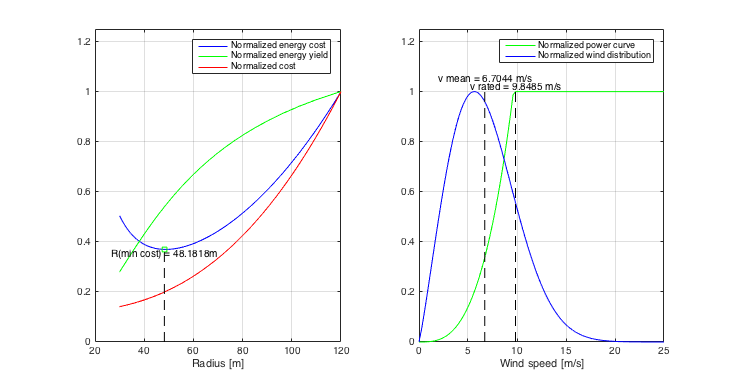
\includegraphics[width=15cm]{Images/op_radius.png}\\